\documentclass[twoside]{book}

% Packages required by doxygen
\usepackage{fixltx2e}
\usepackage{calc}
\usepackage{doxygen}
\usepackage[export]{adjustbox} % also loads graphicx
\usepackage{graphicx}
\usepackage[utf8]{inputenc}
\usepackage{makeidx}
\usepackage{multicol}
\usepackage{multirow}
\PassOptionsToPackage{warn}{textcomp}
\usepackage{textcomp}
\usepackage[nointegrals]{wasysym}
\usepackage[table]{xcolor}

% Font selection
\usepackage[T1]{fontenc}
\usepackage[scaled=.90]{helvet}
\usepackage{courier}
\usepackage{amssymb}
\usepackage{sectsty}
\renewcommand{\familydefault}{\sfdefault}
\allsectionsfont{%
  \fontseries{bc}\selectfont%
  \color{darkgray}%
}
\renewcommand{\DoxyLabelFont}{%
  \fontseries{bc}\selectfont%
  \color{darkgray}%
}
\newcommand{\+}{\discretionary{\mbox{\scriptsize$\hookleftarrow$}}{}{}}

% Page & text layout
\usepackage{geometry}
\geometry{%
  a4paper,%
  top=2.5cm,%
  bottom=2.5cm,%
  left=2.5cm,%
  right=2.5cm%
}
\tolerance=750
\hfuzz=15pt
\hbadness=750
\setlength{\emergencystretch}{15pt}
\setlength{\parindent}{0cm}
\setlength{\parskip}{3ex plus 2ex minus 2ex}
\makeatletter
\renewcommand{\paragraph}{%
  \@startsection{paragraph}{4}{0ex}{-1.0ex}{1.0ex}{%
    \normalfont\normalsize\bfseries\SS@parafont%
  }%
}
\renewcommand{\subparagraph}{%
  \@startsection{subparagraph}{5}{0ex}{-1.0ex}{1.0ex}{%
    \normalfont\normalsize\bfseries\SS@subparafont%
  }%
}
\makeatother

% Headers & footers
\usepackage{fancyhdr}
\pagestyle{fancyplain}
\fancyhead[LE]{\fancyplain{}{\bfseries\thepage}}
\fancyhead[CE]{\fancyplain{}{}}
\fancyhead[RE]{\fancyplain{}{\bfseries\leftmark}}
\fancyhead[LO]{\fancyplain{}{\bfseries\rightmark}}
\fancyhead[CO]{\fancyplain{}{}}
\fancyhead[RO]{\fancyplain{}{\bfseries\thepage}}
\fancyfoot[LE]{\fancyplain{}{}}
\fancyfoot[CE]{\fancyplain{}{}}
\fancyfoot[RE]{\fancyplain{}{\bfseries\scriptsize Generated by Doxygen }}
\fancyfoot[LO]{\fancyplain{}{\bfseries\scriptsize Generated by Doxygen }}
\fancyfoot[CO]{\fancyplain{}{}}
\fancyfoot[RO]{\fancyplain{}{}}
\renewcommand{\footrulewidth}{0.4pt}
\renewcommand{\chaptermark}[1]{%
  \markboth{#1}{}%
}
\renewcommand{\sectionmark}[1]{%
  \markright{\thesection\ #1}%
}

% Indices & bibliography
\usepackage{natbib}
\usepackage[titles]{tocloft}
\setcounter{tocdepth}{3}
\setcounter{secnumdepth}{5}
\makeindex

% Hyperlinks (required, but should be loaded last)
\usepackage{ifpdf}
\ifpdf
  \usepackage[pdftex,pagebackref=true]{hyperref}
\else
  \usepackage[ps2pdf,pagebackref=true]{hyperref}
\fi
\hypersetup{%
  colorlinks=true,%
  linkcolor=blue,%
  citecolor=blue,%
  unicode%
}

% Custom commands
\newcommand{\clearemptydoublepage}{%
  \newpage{\pagestyle{empty}\cleardoublepage}%
}

\usepackage{caption}
\captionsetup{labelsep=space,justification=centering,font={bf},singlelinecheck=off,skip=4pt,position=top}

%===== C O N T E N T S =====

\begin{document}

% Titlepage & ToC
\hypersetup{pageanchor=false,
             bookmarksnumbered=true,
             pdfencoding=unicode
            }
\pagenumbering{roman}
\begin{titlepage}
\vspace*{7cm}
\begin{center}%
{\Large movies \\[1ex]\large 0.\+0.\+1 }\\
\vspace*{1cm}
{\large Generated by Doxygen 1.8.11}\\
\end{center}
\end{titlepage}
\clearemptydoublepage
\tableofcontents
\clearemptydoublepage
\pagenumbering{arabic}
\hypersetup{pageanchor=true}

%--- Begin generated contents ---
\chapter{Hierarchical Index}
\section{Class Hierarchy}
This inheritance list is sorted roughly, but not completely, alphabetically\+:\begin{DoxyCompactList}
\item \contentsline{section}{com.\+mert.\+Genre}{\pageref{classcom_1_1mert_1_1_genre}}{}
\item \contentsline{section}{com.\+mert.\+test.\+Genre\+Test}{\pageref{classcom_1_1mert_1_1test_1_1_genre_test}}{}
\item \contentsline{section}{com.\+mert.\+test.\+Main\+Servlet\+Test}{\pageref{classcom_1_1mert_1_1test_1_1_main_servlet_test}}{}
\item \contentsline{section}{com.\+mert.\+test.\+Update\+D\+B\+Test}{\pageref{classcom_1_1mert_1_1test_1_1_update_d_b_test}}{}
\item Http\+Servlet\begin{DoxyCompactList}
\item \contentsline{section}{com.\+mert.\+Main\+Servlet}{\pageref{classcom_1_1mert_1_1_main_servlet}}{}
\item \contentsline{section}{com.\+mert.\+Save\+Entries}{\pageref{classcom_1_1mert_1_1_save_entries}}{}
\item \contentsline{section}{com.\+mert.\+Search}{\pageref{classcom_1_1mert_1_1_search}}{}
\item \contentsline{section}{com.\+mert.\+Show\+Entries}{\pageref{classcom_1_1mert_1_1_show_entries}}{}
\item \contentsline{section}{com.\+mert.\+Show\+Movies}{\pageref{classcom_1_1mert_1_1_show_movies}}{}
\item \contentsline{section}{com.\+mert.\+Update\+DB}{\pageref{classcom_1_1mert_1_1_update_d_b}}{}
\end{DoxyCompactList}
\end{DoxyCompactList}

\chapter{Class Index}
\section{Class List}
Here are the classes, structs, unions and interfaces with brief descriptions\+:\begin{DoxyCompactList}
\item\contentsline{section}{\hyperlink{classplanets_1_1_main_servlet}{planets.\+Main\+Servlet} }{\pageref{classplanets_1_1_main_servlet}}{}
\end{DoxyCompactList}

\chapter{Class Documentation}
\hypertarget{classcom_1_1mert_1_1_main_servlet}{}\section{com.\+mert.\+Main\+Servlet Class Reference}
\label{classcom_1_1mert_1_1_main_servlet}\index{com.\+mert.\+Main\+Servlet@{com.\+mert.\+Main\+Servlet}}
Inheritance diagram for com.\+mert.\+Main\+Servlet\+:\begin{figure}[H]
\begin{center}
\leavevmode
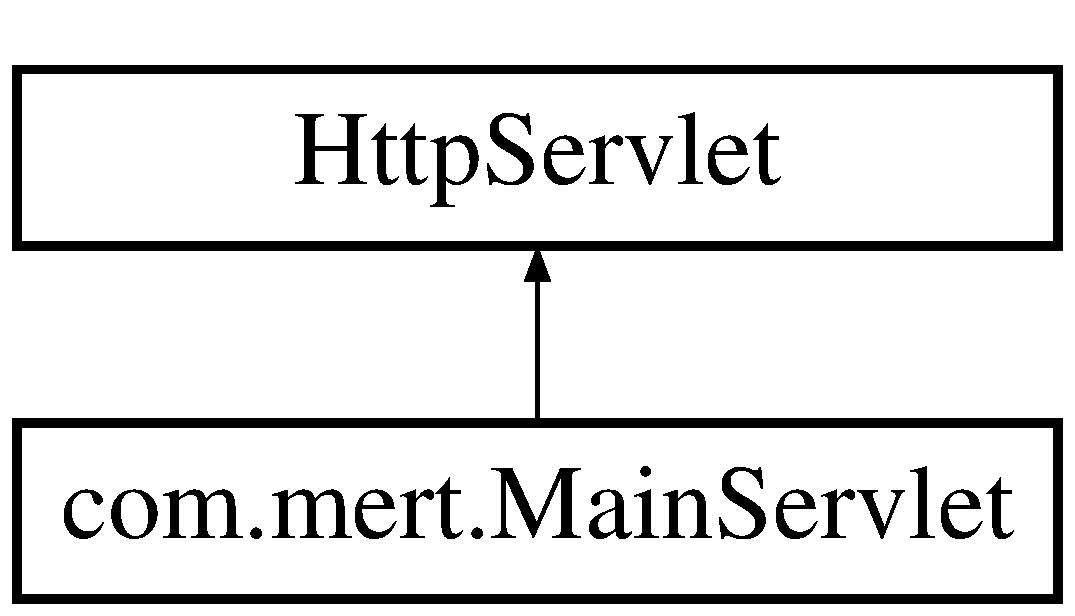
\includegraphics[height=2.000000cm]{classcom_1_1mert_1_1_main_servlet}
\end{center}
\end{figure}
\subsection*{Public Member Functions}
\begin{DoxyCompactItemize}
\item 
\hyperlink{classcom_1_1mert_1_1_main_servlet_a4cd4816907ef657cfb6c7a2403551360}{Main\+Servlet} ()
\item 
void \hyperlink{classcom_1_1mert_1_1_main_servlet_a2f201a8c0bc5b379d4980eae65e774ba}{create\+Movies\+Table} ()
\item 
void \hyperlink{classcom_1_1mert_1_1_main_servlet_a4add4495834801a2cd1aad092e08d2fb}{draw\+Page} (Http\+Servlet\+Request request, Http\+Servlet\+Response response)  throws I\+O\+Exception, Servlet\+Exception, Class\+Not\+Found\+Exception 
\end{DoxyCompactItemize}
\subsection*{Static Public Member Functions}
\begin{DoxyCompactItemize}
\item 
static boolean \hyperlink{classcom_1_1mert_1_1_main_servlet_a44e2c429b5f5c9e74f58d8ec0c044e63}{connect\+To\+DB} ()
\end{DoxyCompactItemize}
\subsection*{Protected Member Functions}
\begin{DoxyCompactItemize}
\item 
void \hyperlink{classcom_1_1mert_1_1_main_servlet_aaff15cf3781104240eb7456c2e249bb5}{do\+Get} (Http\+Servlet\+Request request, Http\+Servlet\+Response response)  throws Servlet\+Exception, I\+O\+Exception 
\item 
void {\bfseries do\+Post} (Http\+Servlet\+Request request, Http\+Servlet\+Response response)  throws Servlet\+Exception, I\+O\+Exception \hypertarget{classcom_1_1mert_1_1_main_servlet_aa028f4c39c100861db897d9d70407249}{}\label{classcom_1_1mert_1_1_main_servlet_aa028f4c39c100861db897d9d70407249}

\end{DoxyCompactItemize}


\subsection{Detailed Description}
\begin{DoxyAuthor}{Author}
Mert Landing page of this web app 
\end{DoxyAuthor}


\subsection{Constructor \& Destructor Documentation}
\index{com\+::mert\+::\+Main\+Servlet@{com\+::mert\+::\+Main\+Servlet}!Main\+Servlet@{Main\+Servlet}}
\index{Main\+Servlet@{Main\+Servlet}!com\+::mert\+::\+Main\+Servlet@{com\+::mert\+::\+Main\+Servlet}}
\subsubsection[{\texorpdfstring{Main\+Servlet()}{MainServlet()}}]{\setlength{\rightskip}{0pt plus 5cm}com.\+mert.\+Main\+Servlet.\+Main\+Servlet (
\begin{DoxyParamCaption}
{}
\end{DoxyParamCaption}
)}\hypertarget{classcom_1_1mert_1_1_main_servlet_a4cd4816907ef657cfb6c7a2403551360}{}\label{classcom_1_1mert_1_1_main_servlet_a4cd4816907ef657cfb6c7a2403551360}
\begin{DoxySeeAlso}{See also}
Http\+Servlet\+::\+Http\+Servlet() 
\end{DoxySeeAlso}


\subsection{Member Function Documentation}
\index{com\+::mert\+::\+Main\+Servlet@{com\+::mert\+::\+Main\+Servlet}!connect\+To\+DB@{connect\+To\+DB}}
\index{connect\+To\+DB@{connect\+To\+DB}!com\+::mert\+::\+Main\+Servlet@{com\+::mert\+::\+Main\+Servlet}}
\subsubsection[{\texorpdfstring{connect\+To\+D\+B()}{connectToDB()}}]{\setlength{\rightskip}{0pt plus 5cm}static boolean com.\+mert.\+Main\+Servlet.\+connect\+To\+DB (
\begin{DoxyParamCaption}
{}
\end{DoxyParamCaption}
)\hspace{0.3cm}{\ttfamily [static]}}\hypertarget{classcom_1_1mert_1_1_main_servlet_a44e2c429b5f5c9e74f58d8ec0c044e63}{}\label{classcom_1_1mert_1_1_main_servlet_a44e2c429b5f5c9e74f58d8ec0c044e63}
Handles all of the sql connections, it is static and is used by other classes too

\begin{DoxyReturn}{Returns}
true if a connection already existed or just established 

false if connection could not be established 
\end{DoxyReturn}
\index{com\+::mert\+::\+Main\+Servlet@{com\+::mert\+::\+Main\+Servlet}!create\+Movies\+Table@{create\+Movies\+Table}}
\index{create\+Movies\+Table@{create\+Movies\+Table}!com\+::mert\+::\+Main\+Servlet@{com\+::mert\+::\+Main\+Servlet}}
\subsubsection[{\texorpdfstring{create\+Movies\+Table()}{createMoviesTable()}}]{\setlength{\rightskip}{0pt plus 5cm}void com.\+mert.\+Main\+Servlet.\+create\+Movies\+Table (
\begin{DoxyParamCaption}
{}
\end{DoxyParamCaption}
)}\hypertarget{classcom_1_1mert_1_1_main_servlet_a2f201a8c0bc5b379d4980eae65e774ba}{}\label{classcom_1_1mert_1_1_main_servlet_a2f201a8c0bc5b379d4980eae65e774ba}
Create movies in local db assuming it does not exist \index{com\+::mert\+::\+Main\+Servlet@{com\+::mert\+::\+Main\+Servlet}!do\+Get@{do\+Get}}
\index{do\+Get@{do\+Get}!com\+::mert\+::\+Main\+Servlet@{com\+::mert\+::\+Main\+Servlet}}
\subsubsection[{\texorpdfstring{do\+Get(\+Http\+Servlet\+Request request, Http\+Servlet\+Response response)}{doGet(HttpServletRequest request, HttpServletResponse response)}}]{\setlength{\rightskip}{0pt plus 5cm}void com.\+mert.\+Main\+Servlet.\+do\+Get (
\begin{DoxyParamCaption}
\item[{Http\+Servlet\+Request}]{request, }
\item[{Http\+Servlet\+Response}]{response}
\end{DoxyParamCaption}
) throws Servlet\+Exception, I\+O\+Exception\hspace{0.3cm}{\ttfamily [protected]}}\hypertarget{classcom_1_1mert_1_1_main_servlet_aaff15cf3781104240eb7456c2e249bb5}{}\label{classcom_1_1mert_1_1_main_servlet_aaff15cf3781104240eb7456c2e249bb5}
This function acts as main and is executed when page is requested.

\begin{DoxySeeAlso}{See also}
Http\+Servlet\+::do\+Get(Http\+Servlet\+Request request, Http\+Servlet\+Response response) 
\end{DoxySeeAlso}
\index{com\+::mert\+::\+Main\+Servlet@{com\+::mert\+::\+Main\+Servlet}!draw\+Page@{draw\+Page}}
\index{draw\+Page@{draw\+Page}!com\+::mert\+::\+Main\+Servlet@{com\+::mert\+::\+Main\+Servlet}}
\subsubsection[{\texorpdfstring{draw\+Page(\+Http\+Servlet\+Request request, Http\+Servlet\+Response response)}{drawPage(HttpServletRequest request, HttpServletResponse response)}}]{\setlength{\rightskip}{0pt plus 5cm}void com.\+mert.\+Main\+Servlet.\+draw\+Page (
\begin{DoxyParamCaption}
\item[{Http\+Servlet\+Request}]{request, }
\item[{Http\+Servlet\+Response}]{response}
\end{DoxyParamCaption}
) throws I\+O\+Exception, Servlet\+Exception, Class\+Not\+Found\+Exception}\hypertarget{classcom_1_1mert_1_1_main_servlet_a4add4495834801a2cd1aad092e08d2fb}{}\label{classcom_1_1mert_1_1_main_servlet_a4add4495834801a2cd1aad092e08d2fb}
Prints out all the html contents on main page such as buttons and search 
\begin{DoxyParams}{Parameters}
{\em request} & \\
\hline
{\em response} & \\
\hline
\end{DoxyParams}

\begin{DoxyExceptions}{Exceptions}
{\em I\+O\+Exception} & \\
\hline
{\em Servlet\+Exception} & \\
\hline
{\em Class\+Not\+Found\+Exception} & \\
\hline
\end{DoxyExceptions}


The documentation for this class was generated from the following file\+:\begin{DoxyCompactItemize}
\item 
src/com/mert/Main\+Servlet.\+java\end{DoxyCompactItemize}

%--- End generated contents ---

% Index
\backmatter
\newpage
\phantomsection
\clearemptydoublepage
\addcontentsline{toc}{chapter}{Index}
\printindex

\end{document}
